\documentclass[12pt]{article}
\usepackage{amsmath, amssymb, amsthm, tikz, pgfplots}
\usepackage{geometry, enumitem, mdframed, array, xcolor, booktabs}
\geometry{margin=1in}

% Custom environments
\newtheorem{definition}{Definition}
\newtheorem{theorem}{Theorem}
\newtheorem{classification}{Classification}
\newtheorem{example}{Example}
\newmdenv[linecolor=blue,linewidth=2pt]{keypoint}
\newmdenv[linecolor=red,linewidth=2pt]{warning}
\newmdenv[linecolor=green,linewidth=2pt]{insight}
\newmdenv[linecolor=purple,linewidth=2pt]{examtip}
\newmdenv[linecolor=orange,linewidth=2pt]{quickcheck}

\title{ODE Lesson 37: 2D Linear Systems: Complete Classification}
\author{ODE 1 - Prof. Adi Ditkowski}
\date{}

\begin{document}
\maketitle

\section{Classification Framework}

Consider the 2D linear system:
$$\dot{\mathbf{x}} = A\mathbf{x}, \quad \text{where } A = \begin{pmatrix} a & b \\ c & d \end{pmatrix}$$

\begin{keypoint}
\textbf{Master Classification Parameters:}
\begin{align}
\text{Trace: } \tau &= \text{tr}(A) = a + d \\
\text{Determinant: } \Delta &= \det(A) = ad - bc \\
\text{Discriminant: } D &= \tau^{2} - 4\Delta
\end{align}
These three quantities completely determine the phase portrait!
\end{keypoint}

\section{Eigenvalue Analysis}

The characteristic equation is:
$$\lambda^{2} - \tau\lambda + \Delta = 0$$

with eigenvalues:
$$\lambda_{1,2} = \frac{\tau \pm \sqrt{\tau^{2} - 4\Delta}}{2} = \frac{\tau \pm \sqrt{D}}{2}$$

\begin{theorem}[Eigenvalue Classification]
The nature of eigenvalues depends on the discriminant $D$:
\begin{itemize}
    \item $D > 0$: Two distinct real eigenvalues
    \item $D = 0$: One repeated real eigenvalue
    \item $D < 0$: Two complex conjugate eigenvalues $\alpha \pm i\beta$
\end{itemize}
\end{theorem}

\section{Complete Classification Table}

\begin{center}
\begin{tabular}{|c|c|c|c|c|}
\hline
\textbf{Type} & \textbf{Condition} & \textbf{Eigenvalues} & \textbf{Stability} & \textbf{Behavior} \\
\hline
\hline
Saddle & $\Delta < 0$ & $\lambda_{1} < 0 < \lambda_{2}$ & Unstable & Hyperbolic \\
\hline
Stable Node & $\Delta > 0, D > 0, \tau < 0$ & $\lambda_{1}, \lambda_{2} < 0$ & Asymp. Stable & Approach \\
\hline
Unstable Node & $\Delta > 0, D > 0, \tau > 0$ & $\lambda_{1}, \lambda_{2} > 0$ & Unstable & Repelling \\
\hline
Stable Spiral & $\Delta > 0, D < 0, \tau < 0$ & $\alpha \pm i\beta, \alpha < 0$ & Asymp. Stable & Spiral in \\
\hline
Unstable Spiral & $\Delta > 0, D < 0, \tau > 0$ & $\alpha \pm i\beta, \alpha > 0$ & Unstable & Spiral out \\
\hline
Center & $\Delta > 0, \tau = 0$ & $\pm i\beta$ & Neutrally Stable & Ellipses \\
\hline
\end{tabular}
\end{center}

\section{Detailed Portrait Descriptions}

\subsection{Saddle Point}

\begin{classification}[Saddle]
\textbf{Condition:} $\det(A) < 0$\\
\textbf{Eigenvalues:} Real with opposite signs\\
\textbf{Key Features:}
\begin{itemize}
    \item Stable manifold: $E^{s} = \text{span}\{v_{1}\}$ where $\lambda_{1} < 0$
    \item Unstable manifold: $E^{u} = \text{span}\{v_{2}\}$ where $\lambda_{2} > 0$
    \item Trajectories approach along $E^{s}$, depart along $E^{u}$
    \item Four hyperbolic sectors
\end{itemize}
\end{classification}

\begin{examtip}
\textbf{Drawing a Saddle:}
\begin{enumerate}
    \item Draw stable eigenvector (arrows pointing in)
    \item Draw unstable eigenvector (arrows pointing out)
    \item Add hyperbolic trajectories in each sector
    \item These are the separatrices - label them!
\end{enumerate}
\end{examtip}

\subsection{Nodes}

\begin{classification}[Proper Node]
\textbf{Condition:} $\Delta > 0$, $D > 0$, $\lambda_{1} \neq \lambda_{2}$\\
\textbf{Behavior:}
\begin{itemize}
    \item All trajectories tangent to slow eigenvector at origin
    \item Fast eigenvector: $|\lambda_{1}| > |\lambda_{2}|$ determines initial direction
    \item Slow eigenvector: determines final approach direction
\end{itemize}
\end{classification}

\begin{classification}[Improper Node]
\textbf{Condition:} $D = 0$, single eigenvector\\
\textbf{Special Case:} $A = \begin{pmatrix} \lambda & 1 \\ 0 & \lambda \end{pmatrix}$ (Jordan form)\\
\textbf{Behavior:} Trajectories curve, all tangent to eigenvector
\end{classification}

\begin{classification}[Star Node]
\textbf{Condition:} $A = \lambda I$ (scalar multiple of identity)\\
\textbf{Behavior:} Straight-line trajectories in all directions
\end{classification}

\subsection{Spirals and Centers}

\begin{classification}[Spiral/Focus]
\textbf{Condition:} $D < 0$ (complex eigenvalues)\\
\textbf{Eigenvalues:} $\lambda = \alpha \pm i\beta$\\
\textbf{Behavior:}
\begin{itemize}
    \item Rotation frequency: $\omega = \beta$
    \item Decay/growth rate: $\alpha$
    \item Clockwise if $\det(A) > 0$ and $b < 0$ (or $c > 0$)
    \item Counterclockwise if $\det(A) > 0$ and $b > 0$ (or $c < 0$)
\end{itemize}
\end{classification}

\begin{insight}
\textbf{Quick Spiral Direction:}
Look at the off-diagonal elements of $A$:
\begin{itemize}
    \item Upper-right positive $(b > 0)$ \rightarrow counterclockwise
    \item Upper-right negative $(b < 0)$ \rightarrow clockwise
\end{itemize}
\end{insight}

\begin{classification}[Center]
\textbf{Condition:} $\tau = 0$, $\Delta > 0$\\
\textbf{Eigenvalues:} Pure imaginary $\pm i\beta$\\
\textbf{Behavior:} Closed elliptical orbits, period $T = 2\pi/\beta$
\end{classification}

\section{Degenerate Cases}

\begin{warning}
\textbf{When $\det(A) = 0$:}
\begin{itemize}
    \item One zero eigenvalue: Line of equilibria
    \item Two zero eigenvalues: Every point is an equilibrium
    \item Parallel trajectories if one eigenvalue is nonzero
\end{itemize}
\end{warning}

\section{The Trace-Determinant Diagram}

\begin{center}
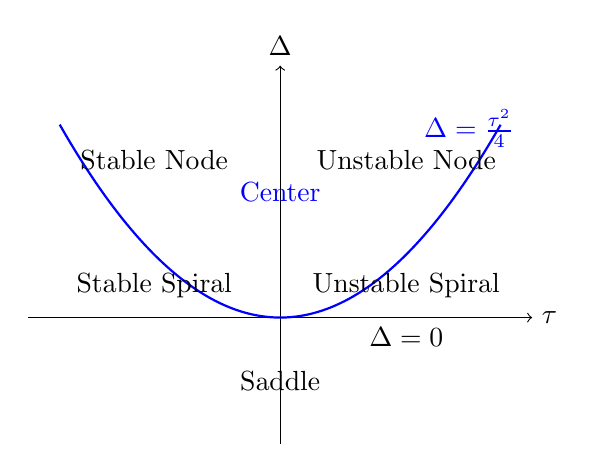
\begin{tikzpicture}[scale=0.8]
    \draw[->] (-4,0) -- (4,0) node[right] {$\tau$};
    \draw[->] (0,-2) -- (0,4) node[above] {$\Delta$};

    % Parabola
    \draw[thick,blue,domain=-3.5:3.5,samples=100] plot (\x, {0.25*\x*\x});

    % Regions
    \node at (-2, 2.5) {Stable Node};
    \node at (2, 2.5) {Unstable Node};
    \node at (-2, 0.5) {Stable Spiral};
    \node at (2, 0.5) {Unstable Spiral};
    \node at (0, -1) {Saddle};
    \node[blue] at (0, 2) {Center};

    % Labels
    \node[blue] at (3, 3) {$\Delta = \frac{\tau^{2}}{4}$};
    \draw[dashed] (-4,0) -- (4,0) node[near end, below] {$\Delta = 0$};
\end{tikzpicture}
\end{center}

\section{Classification Algorithm}

\begin{quickcheck}
\textbf{Prof. Ditkowski's Quick Classification:}
\begin{enumerate}
    \item Compute $\det(A)$
    \begin{itemize}
        \item If $\det(A) < 0$ \rightarrow \textbf{SADDLE} (done!)
        \item If $\det(A) = 0$ \rightarrow Degenerate case
        \item If $\det(A) > 0$ \rightarrow Continue...
    \end{itemize}
    \item Compute $\tau = \text{tr}(A)$
    \begin{itemize}
        \item If $\tau = 0$ \rightarrow \textbf{CENTER}
        \item If $\tau \neq 0$ \rightarrow Continue...
    \end{itemize}
    \item Compute $D = \tau^{2} - 4\det(A)$
    \begin{itemize}
        \item If $D > 0$ \rightarrow \textbf{NODE} (stable if $\tau < 0$)
        \item If $D < 0$ \rightarrow \textbf{SPIRAL} (stable if $\tau < 0$)
        \item If $D = 0$ \rightarrow \textbf{IMPROPER/STAR NODE}
    \end{itemize}
\end{enumerate}
\end{quickcheck}

\section{Examples Gallery}

\begin{example}[Complete Classification]
Classify $A = \begin{pmatrix} 2 & 3 \\ 3 & 2 \end{pmatrix}$:
\begin{align}
\det(A) &= 4 - 9 = -5 < 0
\end{align}
Therefore: \textbf{SADDLE} (unstable)

Verification: $\lambda = \frac{4 \pm \sqrt{16 + 20}}{2} = \frac{4 \pm 6}{2} = 5, -1$ $\checkmark$
\end{example}

\begin{example}[Using Trace-Det Only]
Classify $A = \begin{pmatrix} -3 & 2 \\ -2 & -3 \end{pmatrix}$:
\begin{align}
\tau &= -6 < 0 \quad \text{(stable)} \\
\Delta &= 9 + 4 = 13 > 0 \quad \text{(not a saddle)} \\
D &= 36 - 52 = -16 < 0 \quad \text{(complex eigenvalues)}
\end{align}
Therefore: \textbf{STABLE SPIRAL}
\end{example}

\end{document}